\documentclass{article}

\usepackage[margin=0.75in]{geometry}

\usepackage{polski}
\usepackage[utf8]{inputenc}

\usepackage{graphicx} % Required for inserting images
\usepackage{amsmath}
\usepackage{amssymb}
\usepackage{extpfeil}
\usepackage{float}
\usepackage{matlab-prettifier}
\usepackage{courier}


\usepackage[T1]{fontenc}
%\usepackage{tgbonum}

\title{
    Teoria Sterowania\\
    \Large Metody Częstotliwościowe
}
\author{Maciej Różewicz}
\date{2025}

\makeatletter         
\def\@maketitle{
\raggedright
\begin{center}
    \includegraphics[width=0.5\linewidth]{fig/agh_logo.PNG}\\[8ex]
\end{center}
\begin{center}
    {\huge \bfseries \sffamily \@title }\\[4ex] 
    {\large  \@author}\\[4ex] 
    \@date\\[8ex]
\end{center}}
\makeatother

\begin{document}
\maketitle
\newpage

%%%%%%%%%%%%%%%%%%%%%%%%%%%%%%%%%%%%%%%%%%%%%%%%%%%%%%%%%%%%
\section{Cel ćwiczenia}
Celem ćwiczenia jest analiza stabilności systemów liniowych stacjonarnych za pomocą metod częstotliwościowych.
Będą to dwa kryteria:
\begin{itemize}
    \item kryterium Michajłowa - pozwala określić liczbę pierwiastków stabilnych i~niestabilnych równania charakterystycznego układu na podstawie znajomości jego współczynników,
    \item kryterium Nyquista - pozwala na określenie stabilności układu zamkniętego na podstawie znajomości charakterystyki częstotliwościowej układu otwartego (przy czym warto dodać, że kryterium to działa dla układów o~parametrach skupionych, jak i rozłożonych \cite{Gorecki1993} oraz dla układów z opóźnieniem) - dodatkowo kryterium Nyquista pozwala na określenie liczby pierwiastków w prawej półpłaszczyźnie układu zamkniętego.
\end{itemize}

%%%%%%%%%%%%%%%%%%%%%%%%%%%%%%%%%%%%%%%%%%%%%%%%%%%%%%%%%%%%
\section{Wprowadzenie}
Zanim podane zostaną kryteria badania stabilności układów dynamicznych, przedstawione zostaną pewne pojęcia wprowadzające.

\textbf{Przyrost argumentu}: niech zmienna zespolona $s$ opisuje krzywą $C$ od punktu $s_{1}$ do $s_{2}$ na płaszczyźnie zespolonej.
\begin{figure}[H]
    \centering
    \includegraphics[width=0.5\linewidth]{fig/02_metody_czestotliwosciowe/zasada_argumentu_kontur.PNG}
    \caption{Krzywa $C$ z zasady argumentu.}
    \label{fig:enter-label}
\end{figure}
Niech będzie dana funkcja zmiennej zespolonej $F(s)$.
Gdy zmienna $s$ opisuje krzywą $C$ (przy czym kierunek dodatni obiegu po krzywej $C$ przyjmuje się jako przeciwny do ruchu wskazówek zegara), to funkcja $F(s)$ odwzorowuje krzywą $C$ w krzywą $K$.
Przyrostem argumentu funkcji $F(s)$ - $\Delta _{C}arg F(s)$ - nazywamy kąt opisany przez wektor zaczynający się w początku układu współrzędnych, a którego koniec kreśli krzywą $K$ od punktu $F(s_{1})$ do punktu $F(s_{2})$.
Niech $$F(s) = P(s) + iQ(s)$$ wtedy:
\begin{equation}\label{eq:przyrost_argument}
    \Delta _{C}arg F(s) = \Delta_{C} arg \tan{\left[ \frac{Q(s)}{P(s)} \right]},\,s \in (s_{1}, s_{2})
\end{equation}
\begin{figure}
    \centering
    \includegraphics[width=0.9\linewidth]{fig/02_metody_czestotliwosciowe/zasada_argumentu_kontur_C_K.PNG}
    \caption{Odwzorowanie krzywej $C$ w krzywą $K$.}
    \label{fig:krzywe_odwzorowanie}
\end{figure}

\textbf{Zasada argumentu}: jeżeli funkcja $F(s)$:
\begin{itemize}
    \item jest meromorficzna\footnote{
            Funkcja $f$ jest meromorficzna na danym podzbiorze $D$ płaszczyzny zespolonej, jeśli jest holomorficzna (czyli różniczkowalna w sensie zespolonym) na zbiorze $D/S$, gdzie $S$ jest zbiorem punktów izolowanych, z których każdy jest biegunem funkcji $f$.
        } we wnętrzu domkniętego obszaru $\Omega(s)$, którego brzeg jest pojedynczą krzywą $C$ (ciągłą, bez przecięć i zamkniętą),
    \item jest ciągła i nie posiada zer ani biegunów na krzywej $C$ (tj. na brzegu obszaru $\Omega(s)$)
\end{itemize}
to różnica między ilością zer funkcji $F(s)$ - $Z_{f}$ a ilością biegunów funkcji $F(s)$ - $B_{f}$ we wnętrzu obszaru $\Omega(s)$ ograniczonego krzywą $C$, liczonych ze swoją krotnością, jest równa przyrostowi argumentu:
\begin{equation}\label{eq:zasada_argumentu}
    N = Z_{f} - B_{f} = \frac{1}{2\pi}\Delta_{C}F(s).
\end{equation}
Aby więc obliczyć $N$ trzeba wyznaczyć, ile razy krzywa $K$ obiega początek układu współrzędnych.
Dowód można znaleźć np. w \cite{Gorecki1993}.

Pokazane zostanie tutaj kilka przykładów dla zobrazowania zasady argumentu:
\begin{enumerate}
    \item $F(s) = s -1$ - jeden pierwiastek w konturze
    \begin{figure}[H]
        \centering
        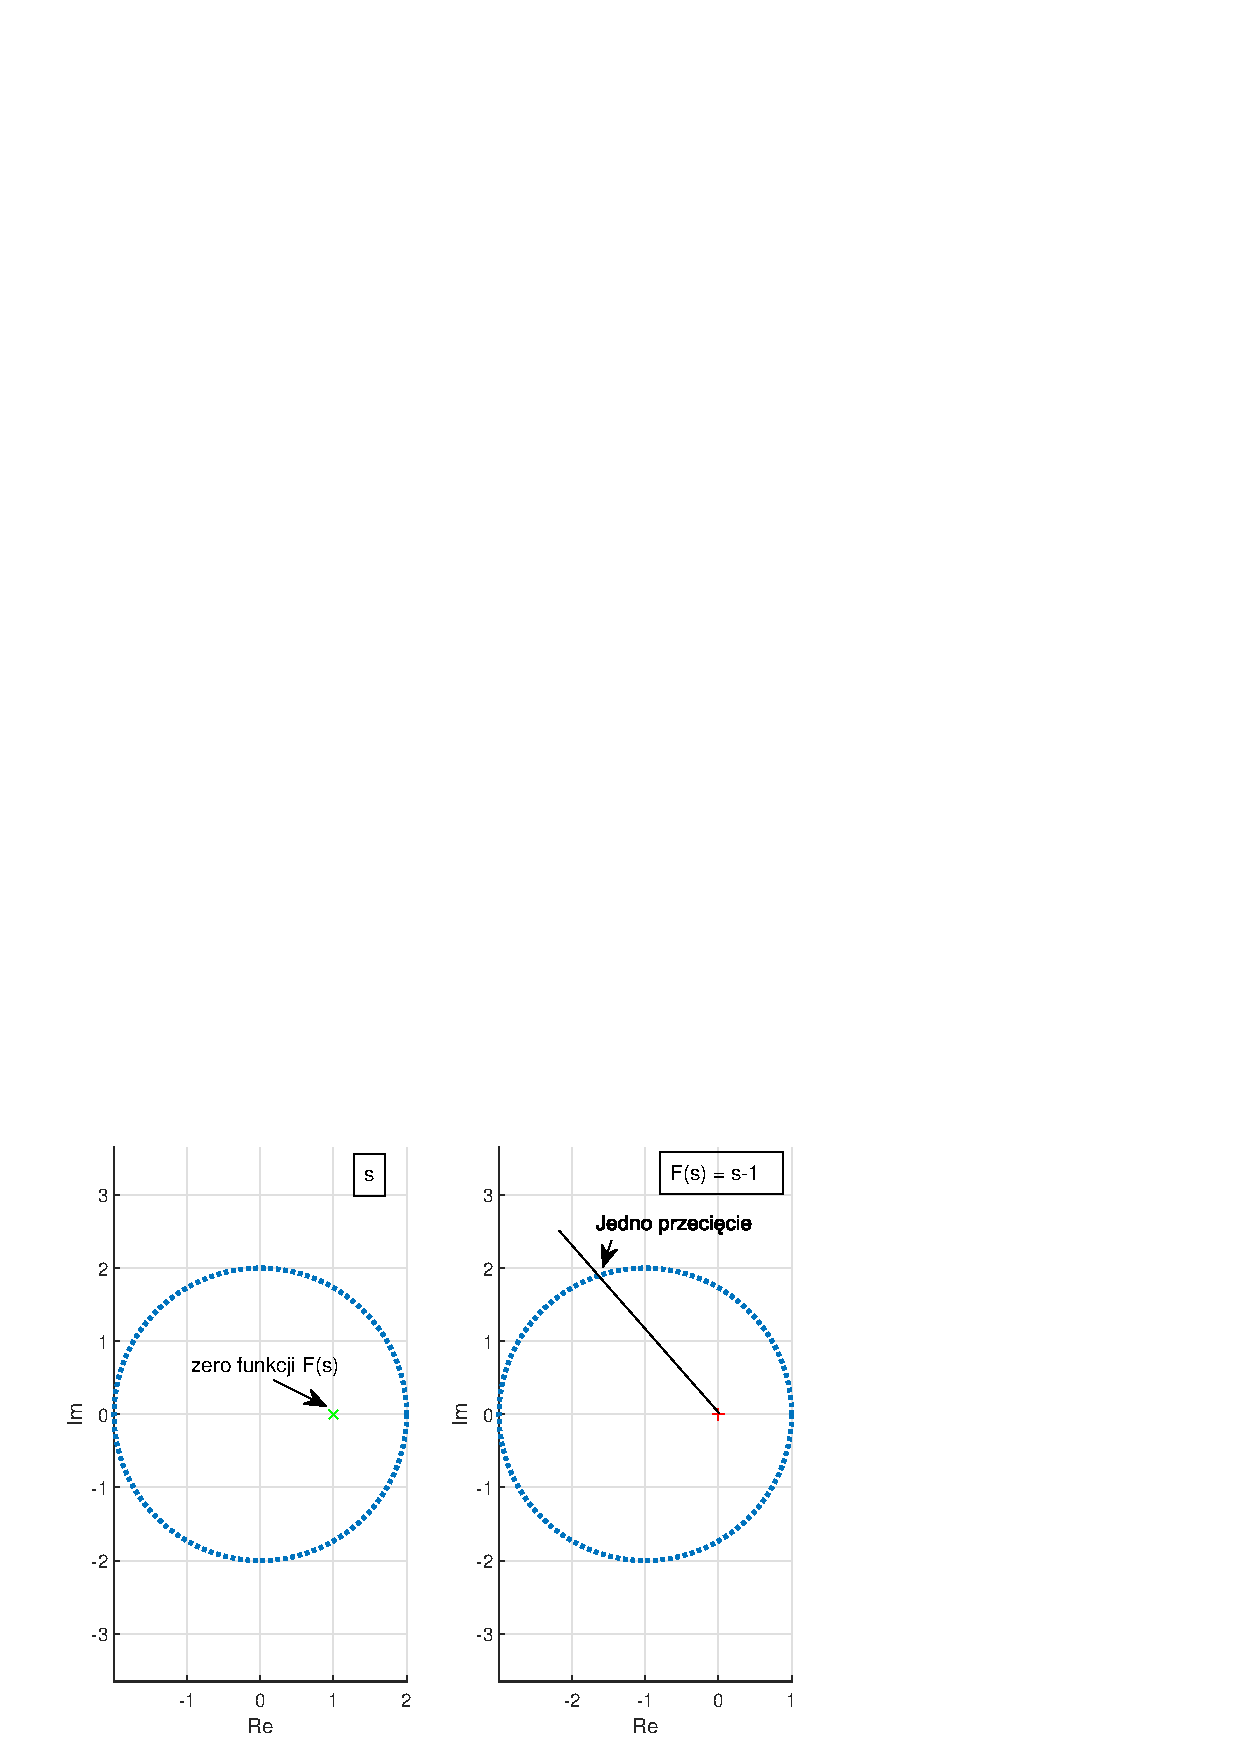
\includegraphics[width=0.7\linewidth]{fig/02_metody_czestotliwosciowe/zasada_argumentu_1.png}
        \caption{Zasada argumentu dla funkcji $F(s) = s-1$ i konturu zdefiniowanego jako okrąg o promieniu 2 i środkiem w punkcie (0,0).}
        \label{fig:enter-label}
    \end{figure}
    \item $F(s) = (s-1)(s-1.55)$  - dwa pierwiastki w konturze
    \begin{figure}[H]
        \centering
        \includegraphics[width=0.7\linewidth]{fig/02_metody_czestotliwosciowe/zasada_argumentu_2.png}
        \caption{Zasada argumentu dla funkcji $F(s) = (s-1)(s-1.55)$ i konturu zdefiniowanego jako okrąg o promieniu 2 i środkiem w punkcie (0,0).}
        \label{fig:enter-label}
    \end{figure}
    \item $F(s) = (s-1)(s-1.55)$  - jeden pierwiastek w konturze
    \begin{figure}[H]
        \centering
        \includegraphics[width=0.7\linewidth]{fig/02_metody_czestotliwosciowe/zasada_argumentu_3.png}
        \caption{Zasada argumentu dla funkcji $F(s) = (s-1)(s-1.55)$ i konturu zdefiniowanego jako okrąg o promieniu 2 i środkiem w punkcie (-0.9,0).}
        \label{fig:enter-label}
    \end{figure}
    \item $F(s) = (s-1)(s-1.55)$  - brak pierwiastków w konturze
    \begin{figure}[H]
        \centering
        \includegraphics[width=0.7\linewidth]{fig/02_metody_czestotliwosciowe/zasada_argumentu_4.png}
        \caption{Zasada argumentu dla funkcji $F(s) = (s-1)(s-1.55)$ i konturu zdefiniowanego jako okrąg o promieniu 2 i środkiem w punkcie (-2.5,0).}
        \label{fig:enter-label}
    \end{figure}
    \item $F(s) = \frac{(s-1)(s-0.5)}{(s-2)(s+0.5)(s+1)(s+0.75)}$  - dwa pierwiastki i cztery bieguny w konturze
    \begin{figure}[H]
        \centering
        \includegraphics[width=0.7\linewidth]{fig/02_metody_czestotliwosciowe/zasada_argumentu_transmitancja.png}
        \caption{Zasada argumentu dla funkcji $F(s) = \frac{(s-1)(s-0.5)}{(s-2)(s+0.5)(s+1)(s+0.75)}$ i konturu zdefiniowanego jako okrąg o~promieniu 3 i środkiem w punkcie (0,0).}
        \label{fig:enter-label}
    \end{figure}
\end{enumerate}

    %=======================================================
    \subsection{Kryterium Michajłowa}
    Jest to kryterium graficzne, pozwalające na zbadanie ilości stabilnych pierwiastków (wraz z krotnościami) wielomianu:
    $$
        H(s) = a_{n}s^{n} + a_{n-1}s^{n-1} + \cdots + a_{1}s + a_{0}
    $$
    Zakłada się, że $H(s)$ nie posiada zer na osi urojonej (jest to założenie potrzebne do konstrukcji odpowiedniego konturu w zasadzie argumentu).
    
    Aby znaleźć liczbę pierwiastków stabilnych (leżących w lewej półpłaszczyźnie zespolonej) można zastosować zasadę argumentu z~obszarem $\Omega(s)$ zdefiniowanym jak na rysunku (\ref{fig:krzywe_odwzorowanie}), gdzie $r \rightarrow \infty$, czyli obejmującym całą lewą półpłaszczyznę.
    Kontur tego obszaru $\Omega(s)$ można opisać jako:
    $$
        \partial \Omega = \left\{ s \in \mathbb{C}: s = i\omega,\omega \in [-r,r] \right\} \cup \left\{ s\in \mathbb{C}: s=re^{i\varphi},\varphi \in [\frac{1}{2}\pi, \frac{3}{2}\pi] \right\}
    $$
    Wówczas, aby sprawdzić liczbę pierwiastków niestabilnych, czy wynosi ona $m$, bada się przyrost argumentu $\Delta_{C} \underset{s\in\partial\Omega}{arg} H(s)$, który powinien wynosić dokładnie $2(n-m)\pi$.

    Badanie przyrostu argumentu na krzywej zamkniętej można podzielić na badanie go na każdej z części tej krzywej, zatem:
    \begin{equation}\label{eq:michajlow_1}
        2(n-m)\pi = \lim_{r\rightarrow\infty}\Delta_{C}\underset{s\in\partial\Omega}{arg}H(s) = 
        \lim_{r\rightarrow\infty}[\Delta_{C} \underset{\omega\in (-\infty,\infty)}{arg} H(i\omega) + \Delta_{C}\underset{s\in\partial\Omega}{arg}H(re^{-i\varphi})]
    \end{equation}
    Dodatkowo można zapisać:
    $$
        \begin{array}{c}
        H(re^{i\varphi}) = a_{n}r^{n}e^{in\varphi} + \cdots + a_{1}re^{i\varphi} + a_{0} = 
        a_{n}r^{n}e^{in\varphi} \left\{ 1 + \frac{a_{n-1}}{a_{n}}\frac{1}{r}e^{-i\varphi} + \cdots + \frac{a_{0}}{a_{n}}\frac{1}{r^{n}}e^{-in\varphi} \right\}
        \end{array}
    $$
    Wówczas:
    $$
        \Delta_{C} \underset{\varphi\in[\frac{1}{2}\pi,\frac{3}{2}\pi]}{arg} \lim_{r\rightarrow\infty} H(re^{i\varphi}) =
        \Delta_{C}\underset{\varphi\in[\frac{1}{2}\pi,\frac{3}{2}\pi]}{arg} \lim_{r\rightarrow\infty} a_{n}r^{n}e^{in\varphi} =
        n[\frac{3}{2}\pi-\frac{1}{2}\pi] = n\pi
    $$
    Podstawiając ostatni wynik do (\ref{eq:michajlow_1}) otrzymuje się:
    $$
        2(n-m)\pi = \Delta_{C} \underset{\omega\in (-\infty,\infty)}{arg} H(i\omega) + n\pi
        \implies
        \Delta_{C} \underset{\omega\in (-\infty,\infty)}{arg} H(i\omega) + n\pi = (n-2m)\pi
    $$
    Ponieważ pierwiastki są symetryczne, możemy rozważać tylko zmianę argumentu od $0$ do $\infty$.

    \textbf{Kryterium Michajłowa} - jeżeli $a_{n} > 0$, to warunkiem dostatecznym i~koniecznym do tego, aby wielomian $H(s)$ miał dokładnie $m$ zer w prawej półpłaszczyźnie zespolonej jest równość:
    \begin{equation}\label{eq:kryterium_michajlowa}
         \underset{\omega \in (0, \infty)}{\Delta arg} H(j\omega) = \frac{1}{2}n\pi - m\pi
    \end{equation}

        %--------------------------------------------------------
        \subsubsection{Przykłady}
        \textbf{Przykład 1} (z \cite{Grabowski2022})
        Dany jest obiekt o transmitancji:
        $$ 
            G(s) = \frac{0.3s^{2} + 2.5s + 65}{0.0024s^{4} + 0.05s^{3} + 8.03s^{2} + 94s + 223}
        $$
        Sprawdzić, czy jest stabilny.
    
        Aby zbadać stabilność układu liniowego wystarczy zbadać rozłożenie pierwiastków wielomianu charakterystycznego:
        $$
            H(s) = 0.0024s^{4} + 0.05s^{3} + 8.03s^{2} + 94s + 223
        $$
        Wyznaczamy funkcje $P(\omega)$ i $Q(\omega)$:
        \begin{itemize}
            \item $P(\omega) = Re(H(j\omega)) = 0.0024\omega^{4} - 8.03\omega^{2} + 223$
            \item $Q(\omega) = Im(H(j\omega)) = -0.05\omega^{3} + 94\omega$
        \end{itemize}
        Aby móc naszkicować plot Michajłowa wystarczy wyznaczyć miejsca zerowe funkcji $P(\omega)$ i $Q(\omega)$ oraz ich znak na odpowiednich przedziałach:
        
        \begin{table}[H]
            \centering
            \begin{tabular}{|c|c|c|c|c|c|c|c|c|}
                \hline
                 $\omega$       & 0     & $\nearrow$  & $\approx$5.29 & $\nearrow$  & $\approx$43.33    & $\nearrow$  & $\approx$57.60    & $\nearrow$\\
                 \hline
                 $P(\omega)$    & 223   & +         & 0     & -         & -         & -         & 0         & +\\
                 \hline
                 $Q(\omega)$    & 0     & +         & +     & +         & 0         & -         & -         & -\\
                 \hline
            \end{tabular}
            \caption{Zmiana wartości funkcji $P(\omega)$ i $Q(\omega)$ - przykład 1.}
            \label{tab:my_label}
        \end{table}
        Sprawdzić jeszcze należy, jak wielomiany zachowują się dla $\omega \rightarrow \infty$, w tym przypadku plot dąży do punktu w~nieskończoności o argumencie $2\pi$.
        Zatem zmiana argumentu wynosi $2\pi = \frac{1}{2}n\pi$, czyli pierwiastki leżą tylko w lewej półpłaszczyźnie, a więc obiekt stabilny.
        \begin{figure}[H]
            \centering
            \includegraphics[width=0.75\linewidth]{fig/02_metody_czestotliwosciowe/michajlow_przyklad_1.PNG}
            \caption{Szkic plotu Michajłowa dla wielomianu $H(s) = 0.0024s^{4} + 0.05s^{3} + 8.03s^{2} + 94s + 223$.}
            \label{fig:enter-label}
        \end{figure}
    
        \textbf{Przykład 2}
        Zbadać ilość niestabilnych pierwiastków wielomianu za pomocą kryterium Michajłowa:
        $$
            H(s) = 0.6s^{5} + 8s^{4} + 21.8s^{3} + 18.4s^{2} + 4s + 9
        $$
        Jak poprzednio bada się wielomiany $P(w)$ i $Q(\omega)$:
        \begin{itemize}
            \item $P(\omega) = Re(H(j\omega)) = 8\omega^{4} - 18.4\omega^{2} + 9$,
            \item $Q(\omega) = Im(H(j\omega)) = 0.6\omega^{5} - 21.8\omega^{3} + 4\omega$.
        \end{itemize}
        Oraz przedziały, na których przyjmują dodatnie lub ujemne wartości:
        
        \begin{table}[H]
            \centering
            \begin{tabular}{|c|c|c|c|c|c|c|c|c|c|c|}
                \hline
                $\omega$   & 0 & $\nearrow$ & $\approx$0.43 & $\nearrow$ & $\approx$0.84 & $\nearrow$ & $\approx$1.26 & $\nearrow$ & $\approx$6.01 & $\nearrow$\\
                \hline
                $P(\omega)$& 9 & + & + & + & 0 & - & 0 & + & + & +\\
                \hline
                $Q(\omega)$& 0 & + & 0 & - & - & - & - & - & 0 & +\\
                \hline
            \end{tabular}
            \caption{Zmiana wartości funkcji $P(\omega)$ i $Q(\omega)$ - przykład 2.}
            \label{tab:my_label}
        \end{table}
        Wyrysowujemy plot Michajłowa:
        \begin{figure}[H]
            \centering
            \includegraphics[width=0.5\linewidth]{fig/02_metody_czestotliwosciowe/michajlow_przyklad_2.PNG}
            \caption{Szkic plotu Michajłowa dla wielomianu $H(s) = 0.6s^{5} + 8s^{4} + 21.8s^{3} + 18.4s^{2} + 4s + 9$.}
            \label{fig:enter-label}
        \end{figure}
        Przyrost argumentu wynosi $\underset{\omega \in (0, \infty)}{\Delta arg}H(j\omega) = \frac{\pi}{2}$, zatem z kryterium Michajłowa otrzymuje się:
        $$
        \underset{\omega \in (0, \infty)}{\Delta arg} H(j\omega) = \frac{\pi}{2} = \frac{5}{2}\pi - m\pi \rightarrow m = 2
        $$
        Zatem wielomian ma 2 pierwiastki w prawej półpłaszczyźnie zespolonej.

    %=======================================================
    \subsection{Kryterium Nyquista}
    Kryterium Nyquista dotyczy badania stabilności układu zamkniętego na podstawie znajomości transmitancji $G_{0}(s)$ / charakterystyki częstotliwościowej układu otwartego.
    \begin{figure}[H]
        \centering
        \includegraphics[width=0.75\linewidth]{fig/02_metody_czestotliwosciowe/nyquist_otwarty_zamkniety.PNG}
        \caption{Układ otwarty i zamknięty dla kryterium Nyquista.}
        \label{fig:enter-label}
    \end{figure}
    Transmitancja układu z zamknięta pętlą sprzężenia zwrotnego ma postać:
    \begin{equation} \label{eq:gz}
        G_{z}(s) = \frac{G_{0}(s)}{1 + G_{0}(s)}
    \end{equation}
    Aby zbadać więc stabilność układu zamkniętego konieczne jest sprawdzenie, czy zera mianownika $G_{z}(s)$, czyli $1 + G_{0}(s)$, zlokalizowane są w lewej półpłaszczyźnie zespolonej.

    \textbf{Kryterium Nyquista} - jeżeli:
    \begin{itemize}
        \item transmitancja układu otwartego ma postać:
        $$
            G_{0}(s) = \frac{L(s)}{s^{k}M(s)}
        $$
        gdzie: $k = 0, 1, 2, \cdots$, $L, M$ - względnie pierwsze wielomiany rzeczywiste zmiennej zespolonej $s$,
        \item $M(s)$ ma $m$ zer w prawej półpłaszczyźnie zespolonej i nie ma zer na osi urojonych,
        \item stopień licznika transmitancji $G_{0}(s)$ jest niższy niż stopień mianownika ($deg(L(s)) < deg(s^{k}M(s))$)
        oraz
        $$
            \frac{L(0)}{M(0)} \neq 0
        $$

        Wówczas warunkiem koniecznym i dostatecznym stabilności układu zamkniętego jest, aby charakterystyka częstotliwościowa układu otwartego, czyli wykres $G(i\omega)$, przy zmianie częstotliwości $\omega$ od $-\infty$ do $+\infty$ okrążała punkt krytyczny $(-1, i0)$ w kierunku dodatnim $m$-razy.
        Innymi słowy przyrost argumentu wektora $G(i\omega)$ względem punktu krytycznego musi wynosić $2m\pi$.
    \end{itemize}

    Dowód podzielimy na dwa przypadki:
    \begin{enumerate}
        \item $G_{0}(s) = \frac{L(s)}{M(s)}$ - bez astatyzmu (pierwiastki $M(s)$ nie leżą na osi urojonych):

        Przyjmując taką postać transmitancji toru otwartego badana transmitancja (badanie ilości zer) $1+G_{0}(s)$ ma postać:
        $$
            1 + G_{0}(s) = \frac{M(s) + L(s)}{M(s)}
        $$
        Aby $G_{z}(s)$ (\ref{eq:gz}) była transmitancją stabilną, wielomian $M(s) + L(s)$ musi mieć wszystkie pierwiastki w lewej półpłaszczyźnie zespolonej.
        Zatem wiedząc, że $M(s) + L(s)$ i $M(s)$ są tego samego stopnia, oraz wiedząc, że $M(s)$ ma $m$ pierwiastków w prawej półópłaszczyźnie, to funkcja $1+G_{0}(s)$ musi mieć $n$ zer w lewej półpłaszczyźnie i $m$ biegunów w prawej półpłaszczyźnie.
        Zatem można zastosować \textbf{zasadę argumentu} z konturem $C$ tak skonstruowanym, aby obejmował całą prawą stronę płaszczyzny zespolonej.
        Kontur ten można skonstruować analogicznie jak do dowodu kryterium Michajłowa.

        Widać zatem, że przyrost argumentu musi wynosić:
        $$
            \underset{\omega \in (-\infty, \infty)}{\Delta arg}[1 + G_{0}(s)] = 2m\pi
        $$

        Formalnie badamy więc transmitancję $1+G_{0}(s)$, ale dodanie jedynki to transmitancji toru otwartego powoduje tylko "przesunięcie jej o jeden" w prawo, zatem zamiast badać przyrost argumentu względem punktu $(0,0)$ transmitancji $1+G_{0}(s)$ można badać przyrost argumentu transmitancji $G_{0}(s)$ wokół punktu $(-1, 0)$. Jest to bardzo praktyczne podejście, gdyż zwykle posiadamy jedynie zdjętą eksperymentalnie charakterystykę obiektu $G(s)$.

        \begin{figure}[H]
            \centering
            \includegraphics[width=1.0\linewidth]{fig/02_metody_czestotliwosciowe/nyquist_stabilny_przeciecia.PNG}
            \caption{Ilustracja kryterium Nyquista dla stabilnego $G_{0}(s)$.}
            \label{fig:enter-label}
        \end{figure}
        \begin{figure}[H]
            \centering
            \includegraphics[width=1.0\linewidth]{fig/02_metody_czestotliwosciowe/nyquist_niestabilny_przeciecia.PNG}
            \caption{Ilustracja kryterium Nyquista dla niestabilnego $G_{0}(s)$ - jeden pierwiastek niestabilny.}
            \label{fig:enter-label}
        \end{figure}
        
        \item $G_{0}(s) = \frac{L(s)}{s^{k}M(s)}$ - posiada astatyzm $k$-tego rzędu:

        W tym przypadku dowód wygląda bardzo podobnie, jednak z powodu istnienia biegunów na osi urojonej konieczne jest zmodyfikowanie konturu $C$, tak by nie zawierał żadnych zer ani biegunów transmitancji $1+G_{0}(s)$.
        Robi się to dodając półokrąg o promieniu $r \rightarrow 0$, jak na rysunku (\ref{fig:nyquist_astatycznyl}).
        \begin{figure}[H]
            \centering
            \includegraphics[width=0.35\linewidth]{fig/02_metody_czestotliwosciowe/nyquist_astatyzm_kontur.png}
            \caption{Kontur wykorzystywany do dowodu kryterium Nyquista z astatyzmem.}
            \label{fig:nyquist_astatycznyl}
        \end{figure}
        Można zatem zapisać:
        $$
            \begin{array}{c}
            2m\pi = \underset{\omega \in (-\infty, \infty)}{\Delta arg}[1 + G_{0}(s)] = lim_{r\rightarrow 0}\underset{\omega \in (\infty,r)}{\Delta arg}[1 + G_{0}(i\omega)] 
            + \underset{\varphi \in [\frac{1}{2}\pi, -\frac{1}{2}\pi]}{\Delta arg}[1 + G_{0}(re^{i\varphi})] +\\
            +\underset{\omega \in (-r,-\infty)}{\Delta arg}[1 + G_{0}(i\omega)] + \lim_{R\rightarrow \infty}\underset{\omega \in (\infty,r)}{\Delta arg}[1 + G_{0}(i\omega)]
            \end{array}
        $$

        Można zauważyć, że "małe" półkole jest odwzorowywane w tor o kierunku ujemnym i promieniu dążącym do nieskończoności, ponieważ:
        $$
            1+G_{0}(re^{i\varphi}) = \frac{L(re^{i\varphi}) + r^{k}e^{ik\varphi}M(re^{i\varphi})}{r^{k}e^{ik\varphi}M(re^{i\varphi})}
        $$
        Czyli przechodząc do granicy otrzymuje się:
        $$
            \underset{r\rightarrow 0}{lim}[1+G_{0}(re^{i\varphi})] = \underset{r\rightarrow 0}{lim}\left[ \frac{L(re^{i\varphi})}{M(re^{i\varphi})}e^{-ik\varphi} \right]r^{-k}\left\{ 1 + \frac{M(re^{i\varphi}r^{k}e^{i\varphi})}{L(re^{i\varphi})} \right\} =
        $$
        $$
            = {\infty} \frac{L(0)}{M(0)}e^{-k\varphi} = \frac{L(0)}{M(0)}\underset{r\rightarrow 0}{lim}\frac{1}{r^{k}}e^{-k\varphi}
        $$
        Zatem tor ten rozpoczyna się w punkcie w nieskończoności o argumencie:
        $$
            arg \frac{L(0)}{M(0)} + k\frac{1}{2}\pi
            =
            \left\{
                \begin{array}{ll}
                     k\frac{1}{2}\pi & dla \frac{L(0)}{M(0)} > 0 \\
                     k\frac{1}{2}\pi - \pi & dla \frac{L(0)}{M(0)} < 0
                \end{array}
            \right\}
        $$
        a kończy na argumencie:
        $$
            arg \frac{L(0)}{M(0)} - k\frac{1}{2}\pi
            =
            \left\{
                \begin{array}{ll}
                     -k\frac{1}{2}\pi & dla \frac{L(0)}{M(0)} > 0 \\
                     -k\frac{1}{2}\pi - \pi & dla \frac{L(0)}{M(0)} < 0
                \end{array}
            \right\}
        $$
        Ostatecznie więc bada się plot $G(i\omega)$ uzupełniony o tor w nieskończoności.

        \begin{figure}[H]
            \centering
            \includegraphics[width=0.75\linewidth]{fig/02_metody_czestotliwosciowe/nyquist_astatyczny.png}
            \caption{Ilustracja kryterium Nyquista dla obiektów z astatyzmem.}
            \label{fig:enter-label}
        \end{figure}
    \end{enumerate}

    Można również udowodnić kryterium Nyquista dla transmitancji w postaci:
    $$
        G_{0}(s) = \frac{L(s)}{(s^{2} + \alpha^{2})M(s)}, \, \alpha\in \mathbb{R}
    $$
    czyli z pierwiastkami na osi urojonej, ale różnymi od 0. Dowód można znaleźć np. w \cite{Grabowski2022}.

        %--------------------------------------------------------
        \subsubsection{Przykłady}
        \textbf{Przykład 3} W pierwszej kolejności rozpatrzmy przypadek, gdy transmitancja układu otwartego jest stabilna:
        \begin{equation}
            G_{0}(s) = \frac{10^{4}}{(s+1)(s+2)(s+3)(s+4)(s+5)(s+6)(s+7)}
        \end{equation}
        Zgodnie z podanym kryterium Nyquista, aby układ zamknięty był stabilny, plot Nyquista nie może ani razu otaczać punktu $(-1, i0)$ (zmiana argumentu musi wynosić 0) - ponieważ liczba pierwiastków niestabilnych układu otwartego wynosi 0.
        Na rysunku (\ref{fig:nyquist_przyklad_stabilny}) przedstawiono plot Nyquista danej transmitancji.
        Łatwo zauważyć, iż ani razu nie okrąża ona punktu krytycznego, zatem po zamknięciu pętli sprzężenia zwrotnego układ regulacji automatycznej będzie stabilny.
        \begin{figure}[H]
            \centering
            \includegraphics[width=1.0\linewidth]{fig/02_metody_czestotliwosciowe/nyquist_stabilny.png}
            \caption{Charakterystyka Nyquista dla układu z przykładu 3.}
            \label{fig:nyquist_przyklad_stabilny}
        \end{figure}
        Warto zauważyć, że w przypadku gdy $G_{0}(s)$ jest stabilne, to potrzebne informacje o kształcie charakterystyki częstotliwościowej uzyskać można również tylko na podstawie charakterystyki Bodego.
        Należy wówczas sprawdzić czy dla fazy -180 stopni magnituda jest mniejsza od 0.
        
        \begin{figure}[H]
            \centering
            \includegraphics[width=1.0\linewidth]{fig/02_metody_czestotliwosciowe/bode_stabilny.png}
            \caption{Charakterystyka Bodego dla układu z przykładu 3.}
            \label{fig:enter-label}
        \end{figure}

        Innym użytecznym typem wykresu jest tak zwany plot Nicholsa. Przedstawia on fazę i magnitudę na jednym wykresie.
        Aby system był stabilny po zamknięciu pętli sprzężenia zwrotnego, plot ten musi okrążać punkt $(-180, 0)$ z prawej strony.
        \begin{figure}[H]
            \centering
            \includegraphics[width=1.0\linewidth]{fig/02_metody_czestotliwosciowe/nichols_stabilny.png}
            \caption{Charakterystyka Nicholsa dla układu z przykładu 3.}
            \label{fig:enter-label}
        \end{figure}
        
        \textbf{Przykład 4} Kolejnym przykładem jest transmitancja niestabilna z jednym pierwiastkiem dodatnim.
        $$
            G_{0}(s) = \frac{15}{(s-1)(s+3)(s+4)}
        $$
        W takim przypadku plot $G_{0}(i\omega)$ musi okrążać punkt $(-1, i0)$ dokładnie jeden raz.
        Na rysunku \ref{fig:przyklad4_bode} widać, że plot Nyquista okrąża punkt krytyczny 1 raz, zatem układ po zamknięciu pętli sprzężenia zwrotnego jest stabilny.
        \begin{figure}[H]
            \centering
            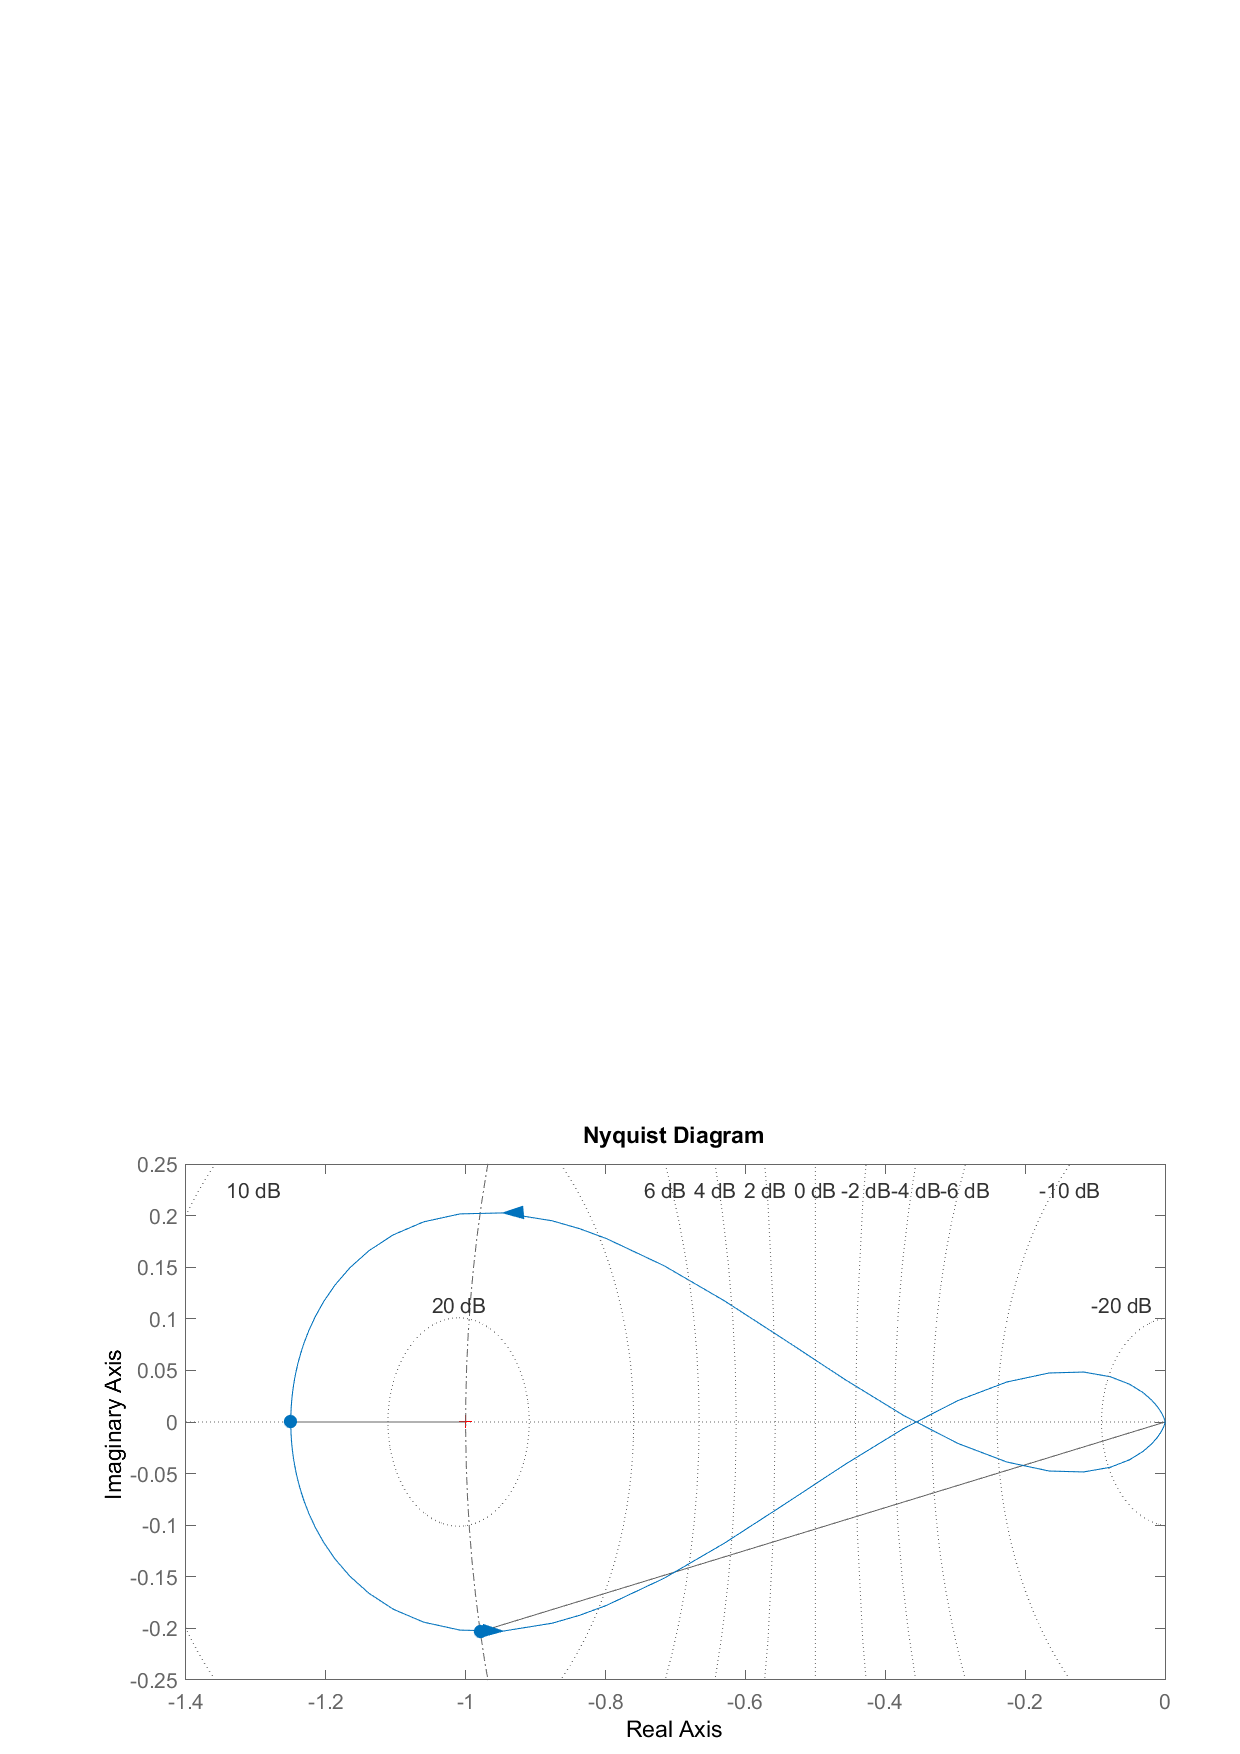
\includegraphics[width=1.0\linewidth]{fig/02_metody_czestotliwosciowe/nyquist_1.png}
            \caption{Charakterystyka Nyquista dla układu z przykładu 3.}
            \label{fig:przyklad4_bode}
        \end{figure}
        W tym przypadku, gdy plot Nyquista przecina oś rzeczywistych kilkukrotnie, to użycie wykresów Bodego nie jest tak oczywiste jak w poprzednim przypadku.
        \begin{figure}[H]
            \centering
            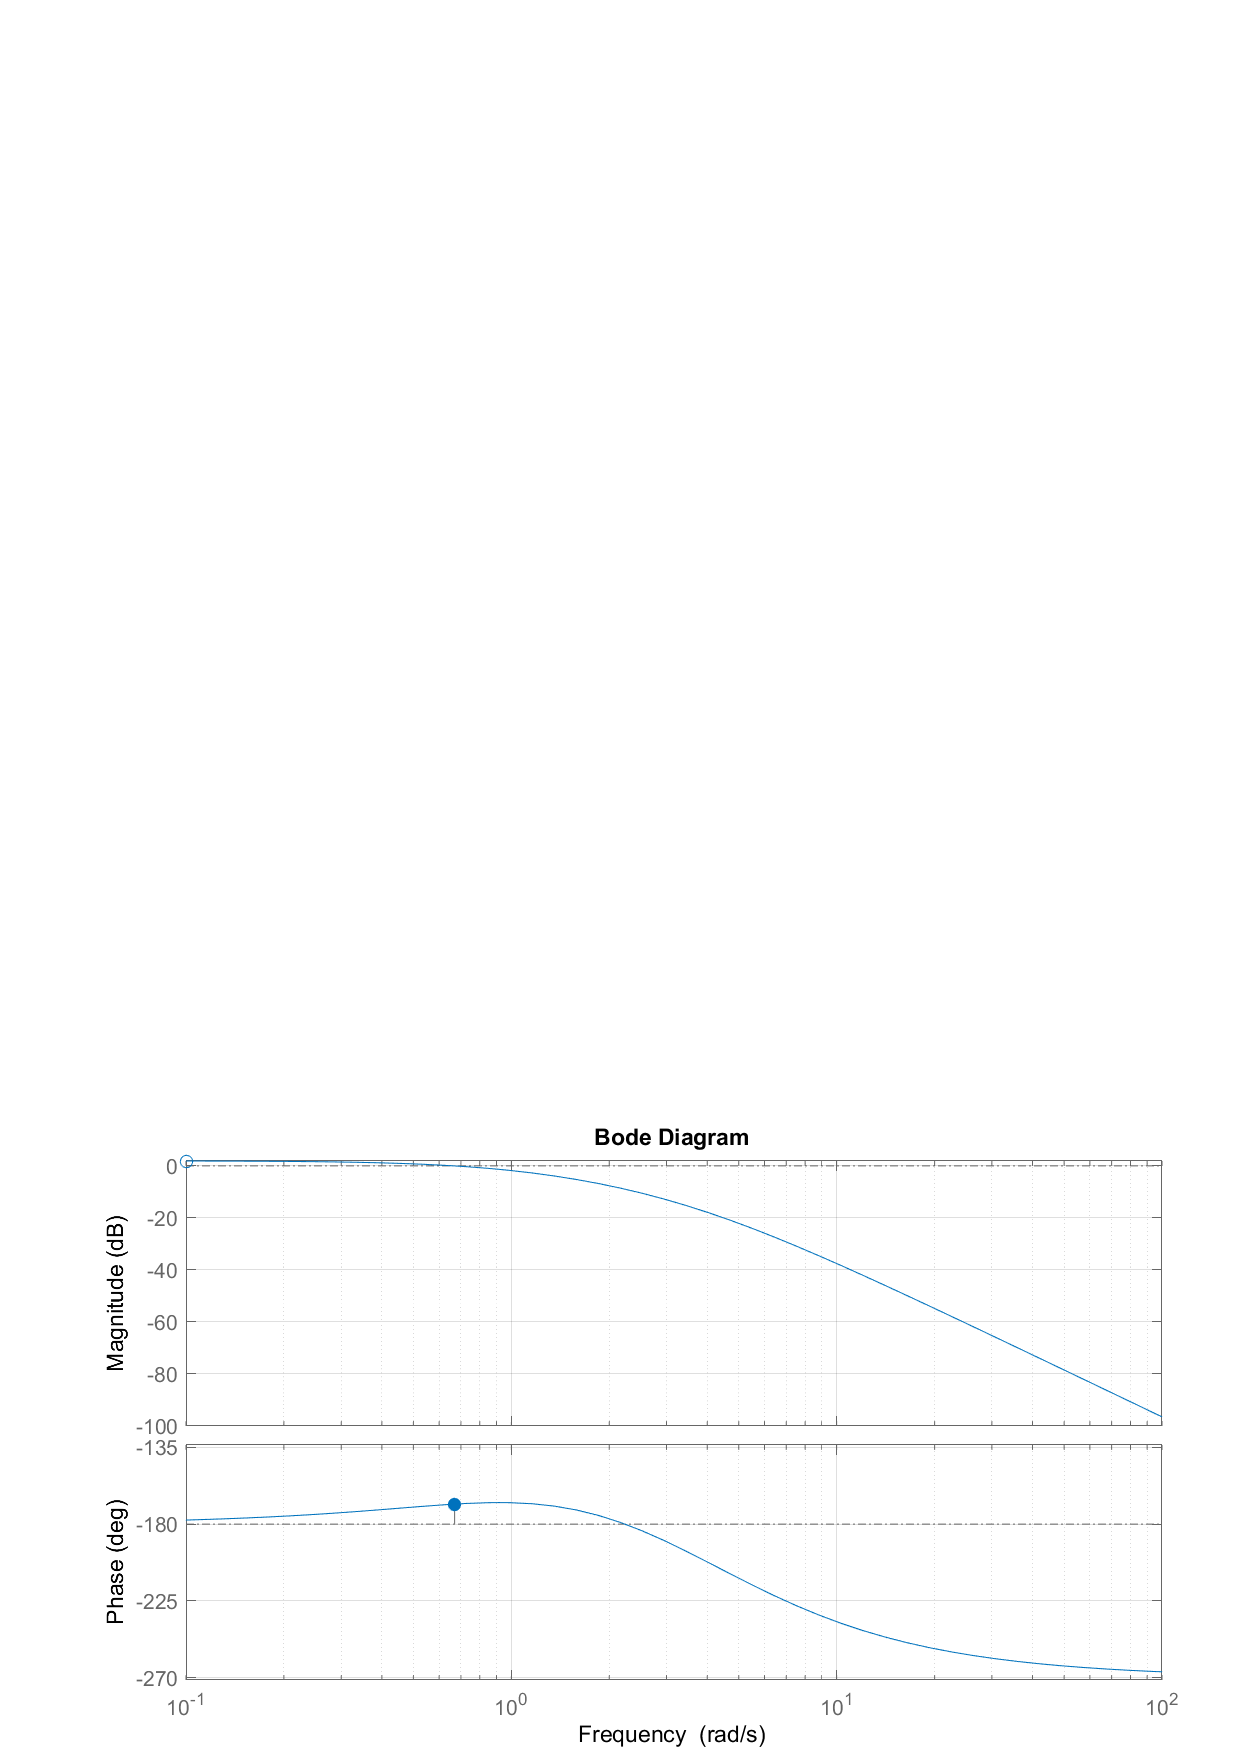
\includegraphics[width=1.0\linewidth]{fig/02_metody_czestotliwosciowe/bode_1.png}
            \caption{Charakterystyka Bodego dla układu z przykładu 3.}
            \label{fig:enter-label}
        \end{figure}
        Natomiast na podstawie plotu Nicholsa możemy również stwierdzić stabilność układu zamkniętego, ponieważ okrąża punkt krytyczny z prawej strony.
        \begin{figure}[H]
            \centering
            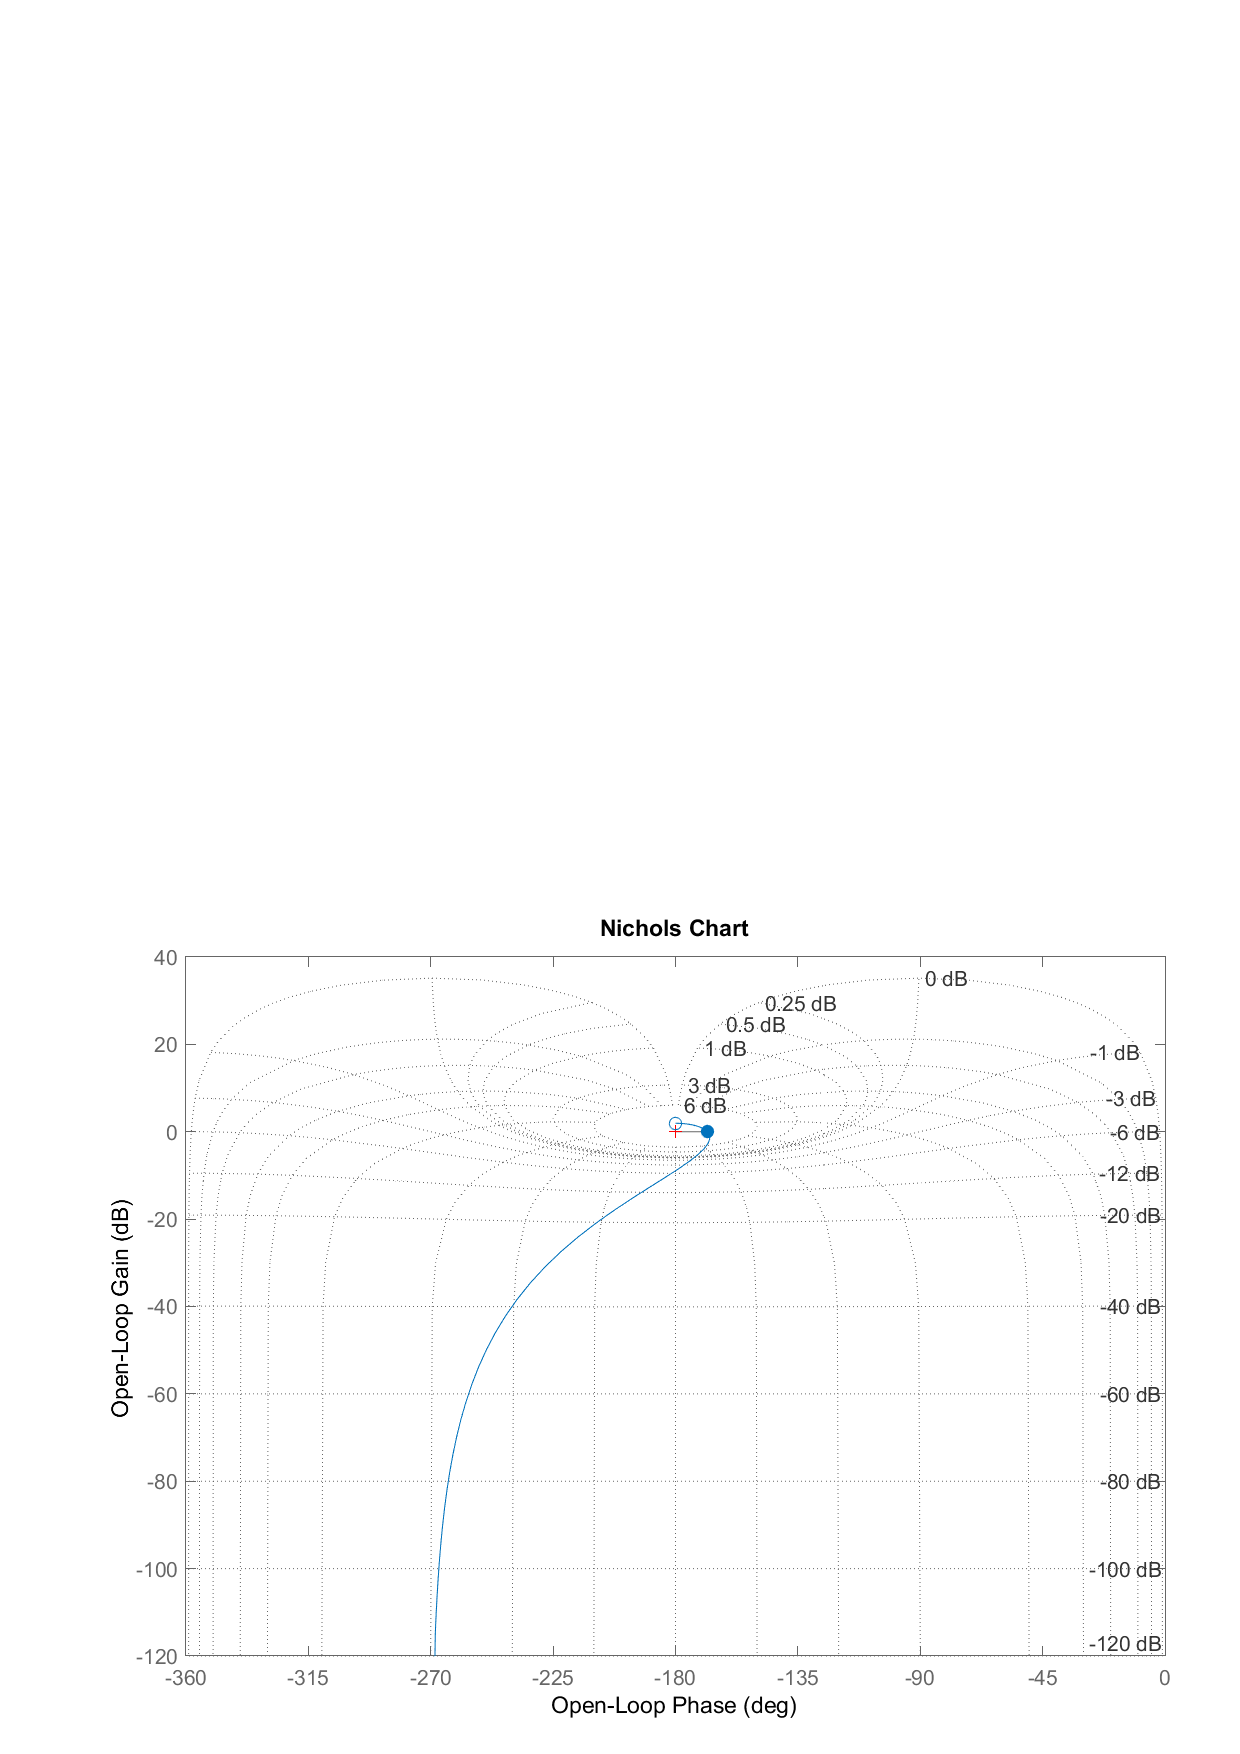
\includegraphics[width=0.75\linewidth]{fig/02_metody_czestotliwosciowe/nichols_1.png}
            \caption{Charakterystyka Nicholsa dla układu z przykładu 3.}
            \label{fig:enter-label}
        \end{figure}
    
        \textbf{Przykład 5}
        W przykładzie tym rozpatrujemy transmitancję $G_{0}(s)$, która posiada jedynie niestabilne pierwiastki.
        $$
            G_{0}(s) = \frac{(s+1)(s+2)(s+3)}{(s-1)(s-2)(s-3)(s-4)}
        $$
        Zatem punkt $(-1, i0)$ musi być okrążony 4-krotnie przez ploty Nyquista.
        \begin{figure}[H]
            \centering
            \includegraphics[width=1.0\linewidth]{fig/02_metody_czestotliwosciowe/nyquist_2.png}
            \caption{Charakterystyka Nyquista dla układu z przykładu 4.}
            \label{fig:enter-label}
        \end{figure}
        Na podstawie plotu Nyquista łatwo zauważyć, że punkt krytyczny nie jest okrążany przez charakterystykę $G_{0}(i\omega)$ ani razu, zatem układ po zamknięciu pętli sprzężenia zwrotnego będzie niestabilny.
        \begin{figure}[H]
            \centering
            \includegraphics[width=1.0\linewidth]{fig/02_metody_czestotliwosciowe/bode_2.png}
            \caption{Charakterystyka Bodego dla układu z przykładu 4.}
            \label{fig:enter-label}
        \end{figure}
        Z plotu Nicholsa widać, iż charakterystyka obiega punkt krytyczny od lewej strony, zatem układ będzie niestabilny.
        \begin{figure}[H]
            \centering
            \includegraphics[width=1.0\linewidth]{fig/02_metody_czestotliwosciowe/nichols_2.png}
            \caption{Charakterystyka Nicholsa dla układu z przykładu 4.}
            \label{fig:enter-label}
        \end{figure}

        Jak można ustabilizować układ zamknięty? Czy można zapewnić stabilizację regulatorem proporcjonalnym?
        \begin{figure}[H]
            \centering
            \includegraphics[width=0.75\linewidth]{fig/02_metody_czestotliwosciowe/zadanie_1.png}
            \caption{Zamknięty układ regulacji.}
            \label{fig:zadanie_}
        \end{figure}
        Po dodaniu regulatora proporcjonalnego transmitancja toru otwartego ma postać:
        $$
            G_{0R}(s) = K\frac{(s+1)(s+2)(s+3)}{(s-1)(s-2)(s-3)(s-4)}
        $$
        Zamiast rozpatrywać całą rodzinę plotów Nyquista, dla każdego $K$ można badać ilość obrotów wokół punktu $(-\frac{1}{K}, i0)$.
        W tym przypadku zauważyć można, że charakterystyka częstotliwościowa okrążać będzie punkt $(-\frac{1}{K}, i0)$ od $K = 10.6878$.

        Znacznie łatwiej w tym przypadku odczytać tę informację z plotu Nicholsa, ponieważ dodanie wzmocnienia oznacza przesunięcie plotu w pionie, a więc sprawdzić o ile trzeba przesunąć wykres w górę, by plot okrążał punkt krytyczny z prawej strony.

        \textbf{Przykład 6}
        Kolejnym przykładem jest obiekt astatyczny z jednym niestabilnym pierwiastkiem równania charakterystycznego.
        $$
            G(s) = \frac{s+1}{s^{3}(s-2)}
        $$
        Ponieważ obiekt jest astatyczny, to plot Nyquista posiada uzupełnienie w nieskończoności.
        Niestety Matlab nie wyrysowuje tego, dlatego trzeba samemu pamiętać o uzpełnieniu.

        W tym przypadku zaczyna się w argumencie $0$, a kończy na $2\pi$.
        Zatem układ jest niestabilny po zamknięciu sprzężenia zwrotnego.
        \begin{figure}[H]
            \centering
            \includegraphics[width=1.0\linewidth]{fig/02_metody_czestotliwosciowe/nyquist_6.png}
            \caption{Charakterystyka Nyquista dla układu z przykładu 6.}
            \label{fig:enter-label}
        \end{figure}
        Identyczne wnioski łatwo wyciągnąć z plotu Nicholsa, gdyż charakterystyka obiega punkt krytyczny z lewej strony.
        \begin{figure}[H]
            \centering
            \includegraphics[width=1.0\linewidth]{fig/02_metody_czestotliwosciowe/nichols_6.png}
            \caption{Charakterystyka Nicholsa dla układu z przykładu 6.}
            \label{fig:enter-label}
        \end{figure}

        \textbf{Przykład 7}
        Ostatnim rozważanym przypadkiem jest transmitancja z członem opóźniającym.
        Nie wpasowuje się ona dokładnie w kształt transmitancji podanej przy sformułowaniu kryterium Nyquista - mimo to jest ono wciąż stosowalne, lecz czasem nazywa się je metodą Cypkina dla tego typu transmitancji.
        $$
            G(s) = \frac{s+1}{(s+2)(s+3)}e^{-s}
        $$
        Mimo innego kształtu transmitancji metoda postępowania jest identyczna - sprawdza się czy plot okrąża punkt krytyczny odpowiednią ilość razy.
        W rozważanym przypadku (rysunek \ref{fig:nyquist_delay}), nie posiadającym niestabilnych pierwiastków, łatwo zauważyć, że plot nie okrąża go ani razu, zatem układ z zamkniętą pętlą sprzężenia zwrotnego będzie stabilny.
        \begin{figure}[H]
            \centering
            \includegraphics[width=1.0\linewidth]{fig/02_metody_czestotliwosciowe/nyquist_7.png}
            \caption{Charakterystyka Nyquista dla układu z przykładu 7.}
            \label{fig:nyquist_delay}
        \end{figure}
        Równie łatwo można dojść do tego samego wniosku analizując plot Nicholsa.
        \begin{figure}[H]
            \centering
            \includegraphics[width=1.0\linewidth]{fig/02_metody_czestotliwosciowe/nichols_7.png}
            \caption{Charakterystyka Nicholsa dla układu z przykładu 7.}
            \label{fig:enter-label}
        \end{figure}
        
%%%%%%%%%%%%%%%%%%%%%%%%%%%%%%%%%%%%%%%%%%%%%%%%%%%%%%%%%%%%
\section{Jak to zrobić w MATLABie?}
Transmitancję w postaci:
$$
    G_{0}(s) = \frac{b_{m}s^{m} + b_{m-1}s^{m-1} + \cdots + b_{1}s + b_{0}}{s^{n} + a_{n-1}s^{n-1} + \cdots + a_{1}s + a_{0}}
$$
Można zdefiniować w MATLABie za pomocą funkcji:
\begin{lstlisting}[style=Matlab-editor]
    G0 = tf([bm bm_1 bm_2 .. b1 b0], [1 an_1 an_2 .. a1 a0])
\end{lstlisting}
Na tak zdefiniowanych transmitancjach można wykonywać działania: $G_{1}(s) \pm G_{2}(s)$, $G_{1}(s) \cdot G_{2}(s)$, $G_{1}(s) / G_{2}(s)$ i~sprzężenie zwrotne $\frac{G_{1}(s)}{1 + G_{1}(s)G_{2}(s)}$ w następujący sposób:
\begin{lstlisting}[style=Matlab-editor]
    G1 = tf([bm1 b1m_1 b1m_2 .. b11 b10], [1 a1n_1 a1n_2 .. a11 a10]);
    G2 = tf([bm2 b2m_1 b2m_2 .. b21 b20], [1 a2n_1 a2n_2 .. a21 a20]);

    G_sum = G1 + G2;
    G_prod = G1 * G2;
    G_div = G1 / G2;
    G_feedback = feedback(G1, G2);
\end{lstlisting}

Jeśli potrzebne jest dodanie opóźnienia - czyli:
$$
    G_{delay}(s) = \frac{b_{m}s^{m} + b_{m-1}s^{m-1} + \cdots + b_{1}s + b_{0}}{s^{n} + a_{n-1}s^{n-1} + \cdots + a_{1}s + a_{0}}e^{-s\tau}
$$
to można to również wykonać za pomocą funkcji \texttt{tf}:
\begin{lstlisting}[style=Matlab-editor]
    G_delay = tf([bm bm_1 bm_2 .. b1 b0], [1 an_1 an_2 .. a1 a0], "OutputDelay", tau)
\end{lstlisting}

Można również zdefiniować zmienną $s$ i później definiować transmitancje już bezpośrednio z jej użyciem, np.:
\begin{lstlisting}[style=Matlab-editor]
    s = tf("s");
    G = (s+1) / (s^2 + 2*s + 1) * exp(-2*s);
\end{lstlisting}

Posiadając zdefiniowaną transmitancję, można wykonać jej ploty: Bodego, Nyquista i Nicholsa:
\begin{lstlisting}[style=Matlab-editor]
    bode_plot = figure();
    bode(s);
    grid on;

    nyquist_plot = figure();
    nyquist(s);
    grid on;

    nichols_plot = figure();
    nichols(s);
    grid on;
\end{lstlisting}

Jeśli interesuje nas konkretny zakres częstotliwości przedstawianych na plotach, to można je podać bezpośrednio do funkcji plotujących (najlepiej zdefiniować je funkcją \texttt{logspace} - zwracającą $n$ punktów rozłożonych w skali logarytmicznej między $10^{x_1}$ a $10^{x_2}$):
\begin{lstlisting}[style=Matlab-editor]
    omega = logspace(x1, x2, n);
    
    bode(s, omega);
    nyquist(s, omega);
    nichols(s, omega);
\end{lstlisting}

%%%%%%%%%%%%%%%%%%%%%%%%%%%%%%%%%%%%%%%%%%%%%%%%%%%%%%%%%%%%
\section{Przebieg ćwiczenia}\
\begin{enumerate}
    \item Rozważamy układ zamknięty z regulatorem proporcjonalnym $G_{R}(s) = K$, przedstawiony na rysunku (\ref{fig:zadanie_1}),
    gdzie transmitancja obiektu sterowanego wynosi:
    $$
        G_{0}(s) = \frac{s+1}{0.01s^{4} + 0.5s^{3} + 3s^{2} - 10s + 10}
    $$
    \begin{figure}[H]
        \centering
        \includegraphics[width=0.75\linewidth]{fig/02_metody_czestotliwosciowe/zadanie_1.png}
        \caption{Zamknięty układ regulacji.}
        \label{fig:zadanie_1}
    \end{figure}
    W czasie laboratorium:
    \begin{itemize}
        \item stosując kryterium Michajłowa wyznaczyć ilość niestabilnych biegunów transmitancji $G_{O}(s)$,
        \item stosując kryterium Nyquista określić wartości współczynnika $K \in \mathbb{R}_{+}$, dla których układ zamknięty będzie stabilny,
        \item wyrysować charakterystykę Bodego i Nicholsa, zaznaczyć zapas fazy i wzmocnienia.
    \end{itemize}
    
    \item Dany jest układ otwarty o transmitancji:
    $$
        G(s) = \frac{4}{s+1}e^{-0.5s}
    $$
    W czasie laboratorium:
    \begin{itemize}
        \item zbadać stabilność układu zamkniętego za pomocą kryterium Nyquista,
        \item sprawdzić, dla jakich wartości $K \in \mathbb{R}_{+}$ regulatora proporcjonalnego układ będzie stabilny,
        \item sprawdzić, dla jakiego opóźnienia układ przestanie być stabilny po zamknięciu pętli sprzężenia zwrotnego.
    \end{itemize}
\end{enumerate}


%%%%%%%%%%%%%%%%%%%%%%%%%%%%%%%%%%%%%%%%%%%%%%%%%%%%%%%%%%%%
\newpage
\begin{thebibliography}{9}

\bibitem{Mitkowski2007}
  Mitkowski W., Baranowski J., Hajduk K., Korytowski A., Tutaj A.,
  \emph{Teoria Sterowania: Materiały Pomocnicze do Ćwiczeń Laboratoryjnych},
  AGH Uczelniane wydawnictwo Naukowo-Dydaktyczne,
  2007.

\bibitem{Amborski1978}
  Amborski K., Marusak A.,
  \emph{Teoria Sterowania w Ćwiczeniach},
  Państwowe Wydawnictwo Naukowe,
  1978.

\bibitem{Gorecki1993}
  Górecki H.,
  \emph{Optymalizacja Systemów Dynamicznych},
  Wydawnictwo Naukowe PWN,
  1993.

\bibitem{Gorecki1971}
  Górecki H.,
  \emph{Analiza i Synteza Układów Regulacji z Opóźnieniem},
  Wydawnictwo Naukowo-Techniczne,
  1971.

\bibitem{Grabowski2022}
  Grabowski P.,
  \emph{Podstawy Teorii Sterowania w Problemach i Zadaniach},
  Wydawnictwo AGH,
  2022.

\bibitem{Nowakowski1999}
  Nowakowski J., Suchomski P.,
  \emph{Teoria Sterowania w Zadaniach},
  Wydawnictwo Politechniki Gdańskiej,
  1999.

\bibitem{Rojtenberg1978}
  Rojtenberg J. N.,
  \emph{Teoria Sterowania},
  Państwowe Wydawnictwo Naukowe,
  1978.

\end{thebibliography}

\end{document}
